%\VignetteIndexEntry{Using MPAgenomics}
\documentclass[a4paper,10pt]{article}
\usepackage[utf8]{inputenc}
\usepackage[T1]{fontenc}
\usepackage{amsmath,amssymb,amsthm}
\usepackage[english]{babel}
\usepackage{graphicx}
\usepackage{geometry}
\usepackage{hyperref}
\usepackage{url}
\usepackage{bibentry}
\geometry{top=3cm, bottom=3cm, left=2cm, right=2cm}

% Title Page
\title{ \texttt{MPAgenomics}: An \texttt{R} package for Multi-Patient Analysis of Genomic Markers.}
\author{Quentin Grimonprez, Samuel Blanck, Alain Celisse, Guillemette Marot}
\date{July, 2014}
\nobibliography*

\usepackage{Sweave}
\begin{document}
\Sconcordance{concordance:MPAgenomics.tex:/home/sblanck/Documents/github/MPAgenomics/vignettes/MPAgenomics.Rnw:%
1 19 1 1 0 56 1 1 2 4 0 2 2 4 0 1 2 3 1 1 2 1 0 7 1 3 0 1 2 3 1 1 2 1 0 %
1 1 3 0 1 2 9 1 1 4 3 0 1 1 3 0 1 2 6 1 1 2 4 0 1 2 13 1 1 4 3 0 1 1 3 %
0 1 2 10 1 1 2 4 0 1 2 3 1 1 4 3 0 1 2 1 0 1 2 4 0 1 2 17 1 1 2 4 0 1 2 %
4 1 1 3 2 0 1 3 2 0 1 2 1 0 1 2 1 0 1 2 1 0 1 2 1 0 1 2 1 0 1 1 3 0 1 2 %
11 1 1 3 2 0 1 2 1 0 1 2 1 0 1 2 1 0 1 4 6 0 1 2 2 1 1 2 1 0 1 2 4 0 1 %
2 5 1 1 2 1 0 1 1 3 0 1 2 2 1 1 3 2 0 1 2 4 0 1 2 9 1 1 3 2 0 1 2 4 0 1 %
2 11 1 1 2 1 0 1 2 4 0 1 2 12 1 1 3 2 0 1 2 4 0 1 2 63 1 1 2 4 0 1 2 %
308 1 1 3 2 0 1 1 1 3 1 0 1 1 3 0 1 2 1 1 1 2 1 0 3 1 3 0 1 2 79 1 1 2 %
1 0 1 2 4 0 1 2 83 1 1 2 1 0 3 1 3 0 1 2 1 1 1 2 4 0 1 2 3 1 1 2 4 0 1 %
2 117 1 1 2 4 0 1 2 72 1 1 5 4 0 1 2 1 0 1 1 3 0 1 2 62 1 1 2 1 0 1 1 3 %
0 1 2 90 1 1 3 2 0 1 2 4 0 1 2 45 1 1 2 1 0 2 1 3 0 1 2 30 1}

\maketitle

\tableofcontents


\section{Introduction}
%	\setkeys{Gin}{width=0.8\textwidth}
		This package provides functions to preprocess and analyze genomic data. Markers refer to SNPs or copy number variations which are designed on the arrays. 
    \texttt{MPAgenomics} is devoted to: $(i)$ efficient segmentation and $(ii)$ genomic marker selection from multi-patient copy number and SNP data profiles.\\
    
    For both types of analyses, a pre-processing step (section \ref{sec:norm}) is proposed as a wrapper of \texttt{aroma.*} packages \cite{aroma}\cite{affy}\cite{aromasite}. 
		This enables to keep maximum information from the original profiles and improve the multi-patient analysis. In particular, this is useful to keep quantitative data for SNPs rather than usual genotype calls (AA, AB or BB) when these states are not relevant (eg in cancer studies where the number of copies differs from two copies). Note that the use of \texttt{aroma.*} packages \cite{aroma} implies that the pre-processing step is only available for Affymetrix DNA chips. The other functionalities of the package \texttt{MPAgenomics} can however be used independently and such procedures are explained in the sections which detail each step of the proposed analysis. 
    
    \texttt{MPAgenomics} suggests an automatic choice of the penalty parameter for the \textsc{Pelt} segmentation \cite{pelt} originally implemented in the \texttt{changepoint} package \cite{peltR}. MPAgenomics also proprose Efficient segmentation with the \textsc{cghseg} segmentation \cite{cghseg}\cite{cghsegb} combined with the slope heuristic \cite{heurpente} to choose automatically the number of segments.\texttt{MPAgenomics} offers a pipeline to perform normalization, segmentation and calling at the same time.
    
    Selection of genomic markers relies on the use of penalized regularization techniques implemented in \texttt{glmnet} \cite{glmnet} and wrappers are offered to relate this package with the normalisation packages. For the users who would like to go further in the use of penalized regularization techniques, we also provide some guidelines to quickly build inputs for the \texttt{HDPenReg} package and interpret some outputs of this latter one.

\section{Preliminaries}

	\subsection{Citing MPAgenomics}
  
  Please always cite the following paper when using \texttt{MPAgenomics}:
    \begin{itemize}
      \item \bibentry{MPAgenomicsHAL}
    \end{itemize}
    
Moreover, \texttt{MPAgenomics} wraps and extends functionalities of several packages. Please try to cite the appropriate methodological papers when you use results from the \texttt{MPAgenomics} software in a publication, as such citations are the main means by which the authors receive professional credit for their work.\\
    
    If you use CRMAv2 normalization in \texttt{MPAgenomics}, please cite:
    \begin{itemize}
      \item \bibentry{CRMAv2}
    \end{itemize}
    
    If you use TumorBoost normalization in \texttt{MPAgenomics}, please cite:
    \begin{itemize}
      \item \bibentry{TumorBoost}
    \end{itemize}
    
    If you use \texttt{MPAgenomics} to segment copy number or allele B fraction profiles with the cghseg segmentation method, please cite:
    \begin{itemize}
      \item \bibentry{cghseg3}
    \end{itemize}
    
    If you use \texttt{MPAgenomics} to segment copy number or allele B fraction profiles with the PELT segmentation method, please cite:
    \begin{itemize}
      \item \bibentry{pelt}
    \end{itemize}
   
    If you use \texttt{MPAgenomics} for calling with \texttt{CGHcall}, please cite:
    \begin{itemize}
      \item \bibentry{CGHcall}
    \end{itemize}
    
  \subsection{Installation}
		The package can be installed either from a GUI (selecting the R-forge repository) or with the command line (to be typed in the R console)
\begin{Schunk}
\begin{Sinput}
> install.packages("MPAgenomics", repos="http://R-Forge.R-project.org")
\end{Sinput}
\end{Schunk}
		This vignette can be produced with the command
\begin{Schunk}
\begin{Sinput}
> vignette("MPAgenomics")
\end{Sinput}
\end{Schunk}
	
		
		Since the package provides simple wrappers of many existing packages and all users are not interested by the same wrappers, we did not force \texttt{MPAgenomics} to depend on all the packages. We however recommend the user who would like to preprocess data to install \texttt{aroma} packages \cite{aroma} with the following commands:
	
\begin{scriptsize}
\begin{Schunk}
\begin{Sinput}
> source("http://www.braju.com/R/hbLite.R")
> hbLite("sfit")
> source("http://bioconductor.org/biocLite.R")
> biocLite("affxparser")
> biocLite("DNAcopy")
> biocLite("aroma.light")
> install.packages("aroma.affymetrix")
> install.packages("aroma.cn")
\end{Sinput}
\end{Schunk}
\end{scriptsize}

We also recommend the user who would like to use the cghseg segmentation method to install \texttt{cghseg} package \cite{cghseg} with the following commands:
\begin{scriptsize}
\begin{Schunk}
\begin{Sinput}
> drat::addRepo("sblanck")
> install.packages("cghseg")
\end{Sinput}
\end{Schunk}
\end{scriptsize}


		The installation of all these packages at the very beginning of the use of \texttt{MPAgenomics} is only for convenience, not mandatory. Indeed, the user who would have forgotten to install some packages would be reminded to install them when applying the corresponding wrapper.
	
\section{Starting example}

		This introductory example aims at helping the user understand the main functions of the package. For more details on each step, we invite the user to read the appropriate section. 
	
		\subsection{Download a toy data-set}	
	
			The example is based on a free data-set containing 8 .CEL files (251Mo) which can be downloaded from the Broad Institute website, following this link:
			\url{http://www.broadinstitute.org/mpg/birdsuite/downloads/birdsuite_inputs_1.5.3.tgz}
			If you are used to decompress .tgz files, extract this file and copy the following command in the R console, replacing the path to the directory where the raw data (.CEL files) are stored with the appropriate one. Note that we deliberately use ``/'' and not ``$\backslash$'' in \texttt{celPATH}. If you copy paste paths from Windows (e.g. looking at properties of the directory), you must change ``$\backslash$'' by ``/'' or ``$\backslash\backslash$''.
	
\begin{Schunk}
\begin{Sinput}
> celPATH="/home/user/Documents/workdir/CELdata/cel"
\end{Sinput}
\end{Schunk}

In this example, the directory pointed by celPATH must contain the files shown in Figure \ref{dfSingle2}.

			\begin{figure}[!h]
				\centering
				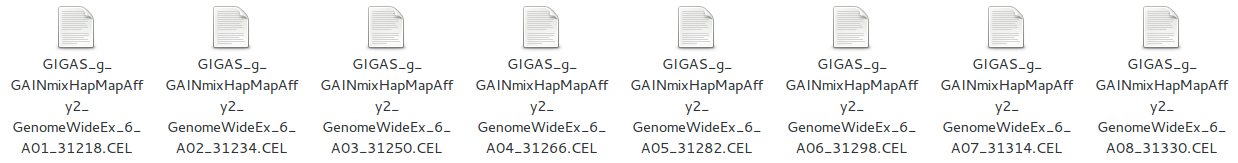
\includegraphics[width=0.9\textwidth]{fig/dataFilesSingle2}
				\caption{CEL files in \texttt{celPATH} (variable containing the path to the downloaded CEL files).}
				\label{dfSingle2}
			\end{figure}
	
			If it is not the case, e.g. if you do not know how to download and extract .tgz files (e.g. via a right click) , you can use the following commands in the R console:
	
	
			\begin{scriptsize}
\begin{Schunk}
\begin{Sinput}
> #set your working directory (replace with the appropriate path)
> workdir="/home/user/Documents/workdir"
> setwd(workdir)
> #download file
> download.file("http://www.broadinstitute.org/mpg/birdsuite/downloads/birdsuite_inputs_1.5.3.tgz",
+ destfile="./CELdata.tgz")
> #untar the file
> untar("./CELdata.tgz",files="cel",exdir=".")
> #indicate the path containing .cel files
> celPATH="./cel"
\end{Sinput}
\end{Schunk}
			\end{scriptsize}


			Once .CEL files are extracted, you must download all the GenomeWideSNP\_6 annotation files which are needed to pre-process the data. These files have extensions .cdf, .ufl, .ugp, .acs. 
			You can download the cdf files (258Mo) from the Affymetrix website (an user account is required), following this link 
			\begin{small}
					\url{http://www.affymetrix.com/Auth/support/downloads/library_files/genomewidesnp6_libraryfile.zip}
			\end{small}
		
			Extract these files and replace the following path with the appropriate one pointing to the folder containing the extracted .cdf files (only GenomeWideSNP\_6.Full.cdf is needed but you can leave the other files in the same folder):	
		
\begin{Schunk}
\begin{Sinput}
> chipPATH="/home/user/Documents/workdir/CD_GenomeWideSNP_6_rev3/Full/GenomeWideSNP_6/LibFiles/"
\end{Sinput}
\end{Schunk}
			
			If you do not know how to decompress .zip files, you can use the following commands in the R console for convenience:
	
			\begin{scriptsize}
\begin{Schunk}
\begin{Sinput}
> #unzip required files
> unzip("./genomewidesnp6_libraryfile.zip",
+  files=c("CD_GenomeWideSNP_6_rev3/Full/GenomeWideSNP_6/LibFiles/GenomeWideSNP_6.Full.cdf"),exdir=".")
> #indicate the path containing .cdf files
> chipPATH="./home/user/Documents/workdir/CD_GenomeWideSNP_6_rev3/Full/GenomeWideSNP_6/LibFiles/"
\end{Sinput}
\end{Schunk}
			\end{scriptsize}

		
			The other annotation files can be downloaded from \url{http://www.aroma-project.org/data/annotationData/chipTypes/GenomeWideSNP_6/}. For this example, we download GenomeWideSNP\_6,Full,na31,hg19,HB20110328.ufl.gz (6Mo), GenomeWideSNP\_6,Full,na31,hg19,HB20110328.ugp.gz (7Mo), GenomeWideSNP\_6,HB20080710.acs.gz (37Mo). Extract these files in the folder where your cdf files are in order to have all the annotation files in the same folder (see Figure \ref{chipfileinit}).

			\begin{figure}[!h]
				\centering
				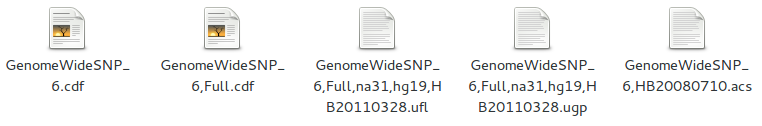
\includegraphics[width=0.6\textwidth]{fig/chipFiles2}\\
				\caption{Chip GenomeWideSNP\_6 files in \texttt{chipPATH} (variable containing the path to the downloaded chip files).}%\texttt{./Documents/chips/SNP6}.}
				\label{chipfileinit}
			\end{figure}			
			

%			Because names of cdf files in the aroma architecture must have the following format: \\
%			<chip type>,<tags>.cdf.
		
%			So, we have to change \texttt{GenomeWideSNP\_6.Full.cdf} into \texttt{GenomeWideSNP\_6,Full.cdf}.
%			\begin{small}
%				\begin{verbatim}
%			chipPATH=paste0(exdirChip,"/CD_GenomeWideSNP_6_rev3/Full/GenomeWideSNP_6/LibFiles/")
%			renameFile(paste0(chipPATH,"GenomeWideSNP_6.Full.cdf"),paste0(chipPATH,"GenomeWideSNP_6,Full.cdf"))
%				\end{verbatim}
%			\end{small}
%		cela devrait etre inclus dans l'architecture		
	
			If you do not know how to download or decompress .gz files, you can use the following commands in the R console for convenience:
	
			\begin{scriptsize}
\begin{Schunk}
\begin{Sinput}
> #set the directory where the .cdf files are as your working directory 
> setwd(chipPATH) 	
> ##download the 3 files .ufl, .ugp, .acs
> download.file("http://www.aroma-project.org/data/annotationData/chipTypes/GenomeWideSNP_6/GenomeWideSNP_6,Full,na31,hg19,HB20110328.ufl.gz",
+ destfile="GenomeWideSNP_6,Full,na31,hg19,HB20110328.ufl.gz")
> download.file("http://www.aroma-project.org/data/annotationData/chipTypes/GenomeWideSNP_6/GenomeWideSNP_6,Full,na31,hg19,HB20110328.ugp.gz",
+ destfile="GenomeWideSNP_6,Full,na31,hg19,HB20110328.ugp.gz")
> download.file("http://www.aroma-project.org/data/annotationData/chipTypes/GenomeWideSNP_6/GenomeWideSNP_6,HB20080710.acs.gz", 
+ destfile="GenomeWideSNP_6,HB20080710.acs.gz")
> #unzip the gz files
> #install R.utils package containing the gunzip function
> install.packages("R.utils")
> library("R.utils")
> gunzip("GenomeWideSNP_6,Full,na31,hg19,HB20110328.ufl.gz",
+ destname="GenomeWideSNP_6,Full,na31,hg19,HB20110328.ufl")
> gunzip("GenomeWideSNP_6,Full,na31,hg19,HB20110328.ugp.gz",
+ destname="GenomeWideSNP_6,Full,na31,hg19,HB20110328.ugp")
> gunzip("GenomeWideSNP_6,HB20080710.acs.gz",destname="GenomeWideSNP_6,HB20080710.acs")
\end{Sinput}
\end{Schunk}
			\end{scriptsize}


		\subsection{Use of the main functions of the package}	
			\label{mainuse}
        		In the following example, we suggest to perform segmentation and calling before selection of markers even if only the pre-processing step, which estimates the copy-number and the allele B fraction profile, is required for the last one.

        		We assume that all the required chip files are in the \texttt{chipPATH} folder and that the .CEL files are in the \texttt{celPATH} folder.


			First, we normalize .CEL files using the CRMAv2 method \cite{CRMAv2} from aroma packages. These packages require a specific architecture containing .CEL and annotation files. This normalization step is required before any statistical analysis. The following command performs the creation of architecture and the normalization at the same time:
			
\begin{Schunk}
\begin{Sinput}
> #list files to check that your path to annotation files (.cdf, .ugp, .ufl, .acs) is correctly set
> dir(chipPATH)
> # list files to check that your path to cel files (.cel) is correctly set
> dir(celPATH) 
> #set your working directory (where you have rights to write)
> setwd(workdir) 
> #normalize data (might take several hours)
> signalPreProcess(dataSetName="datatest1", chipType="GenomeWideSNP_6",
+ dataSetPath=celPATH,chipFilesPath=chipPATH, path=".",
+ createArchitecture=TRUE, savePlot=TRUE, tags="Full")
\end{Sinput}
\end{Schunk}
	
			The first pipeline offered in \texttt{MPAgenomics} consists in the segmentation of every copy-number profile of the data. Then, a calling method can be applied on all the segments to label them (e.g. ``loss'', ``normal'', ``gain''). To perform segmentation and calling at the same time, type the following lines in your R console:

\begin{Schunk}
\begin{Sinput}
> segcall=cnSegCallingProcess("datatest1",chromosome=c(1,5),method="PELT")
> #summary of segmentation and calling process
> segcall
\end{Sinput}
\end{Schunk}

			In this example, chromosomes 1 and 5 for all patients are studied. Figures can be found at \texttt{./figures/datatest1/segmentation/}. 
			To better understand the way the results have been produced, we refer to sections \ref{sec:norm}, \ref{sec:seg} and \ref{sec:calling}.
	
			Results of the calling can be filtered to keep only segments of a minimal size or with a specific label. For example, if you want to only keep segments which represent losses or gains with a minimal size of $10$pb and containing at least 2 probes, run the following command:  
	
\begin{Schunk}
\begin{Sinput}
> callfiltered=filterSeg(segcall,minLength=10,minProbes=2,keptLabel=c("gain","loss"))
> head(callfiltered)
\end{Sinput}
\end{Schunk}
	
			To perform selection of markers, a response is associated with each profile and the goal is to find the most relevant markers in the profile according to the response. You can run the following commands:

\begin{Schunk}
\begin{Sinput}
> dataResponse=data.frame(files=getListOfFiles("datatest1"),
+ response=c(2.105092,1.442868,1.952103,1.857819,2.047897,1.654766,2.385327,2.113406))
> res=markerSelection("datatest1",dataResponse,chromosome=21:22,signal="CN",
+ onlySNP=TRUE,loss="linear")
\end{Sinput}
\end{Schunk}


			For interpretation of all the results, we refer to section \ref{sec:select}.

		\subsection{To go further\dots}

			\paragraph{Use of control samples}
  \label{mainusecontrol}
				In the previous example, there was no control sample. By default, the median of all the samples is used as a reference to estimate the copy-number profile. It is generally better to provide control samples. When this is the case, it is necessary to provide a file or a data.frame giving the correspondence between each control and each sample. For this example, we assume that the control is arbitrarily the first file:

\begin{Schunk}
\begin{Sinput}
> #get the file names of our data-set
> files=getListOfFiles("datatest1")
> #create the data.frame linking normal and tumor files
> normalTumorArray=data.frame(normal=rep(files[1],7),tumor=files[2:8])
\end{Sinput}
\end{Schunk}
	
				\begin{figure}[!h]
					\centering
					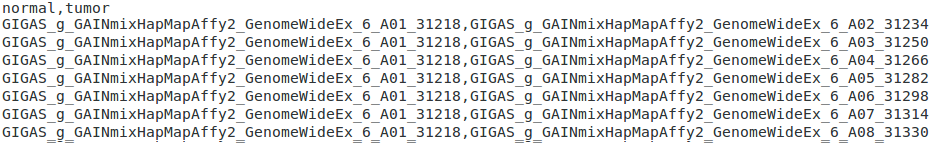
\includegraphics[width=0.8\textwidth]{fig/normalTumorArrayExample}
					\caption{CSV file linking normal sample with tumoral sample.}
				\end{figure}

				Note that the extension .CEL is not provided in the \texttt{normalTumorArray} dataframe.
				In the following of the vignette, a study which provides both control and tumoral samples will be refered as a normal-tumor study.
				
				A new normalization can be run by taking into account information from the control sample. To separate analyses with or without control samples, we will store results from this normal-tumor study under the name ``datatest2''. As the architecture has already been created for ``datatest1'', it is not necessary to run \texttt{signalPreProcess} with \mbox{\texttt{createArchitecture=TRUE}}. It is faster to add the CEL files in ``datatest2'' while leaving the chip definition files as they are by using the function \texttt{addData} and then \texttt{signalPreProcess} with \mbox{\texttt{createArchitecture=FALSE}}.

\begin{Schunk}
\begin{Sinput}
> addData(dataSetName="datatest2",dataPath=celPATH,chipType="GenomeWideSNP_6")
> signalPreProcess(dataSetName="datatest2", chipType="GenomeWideSNP_6",
+ normalTumorArray=normalTumorArray, createArchitecture=FALSE, savePlot=TRUE, tags="Full")
\end{Sinput}
\end{Schunk}
			\paragraph{Single-Patient Analysis of allele B fraction}

				The segmentation example (\ref{mainuse}) was run on the copy-number profile, the allele B fraction can also be segmented after some transformation but only heterozygous SNPs are kept. First, a naive genotype call \cite{TumorBoost} is performed on each normal sample in order to separate heterozygous SNPs from homozygous SNPs. Naive genotyping method assumes SNPs are bi-allelic and therefore is not recommended for tumor samples. Thus allele B fraction segmentation in \texttt{MPAgenomics} requires matched normal-tumor pairs. Then, the resulting signal is symmetrized around 0.5 (a point $x$ become $2 * |x - 0.5|$) \cite{mBAF}(see Figure \ref{figsymFracB}), which makes it similar to the usual copy number.
        
				\begin{figure}[!h]
					\centering
					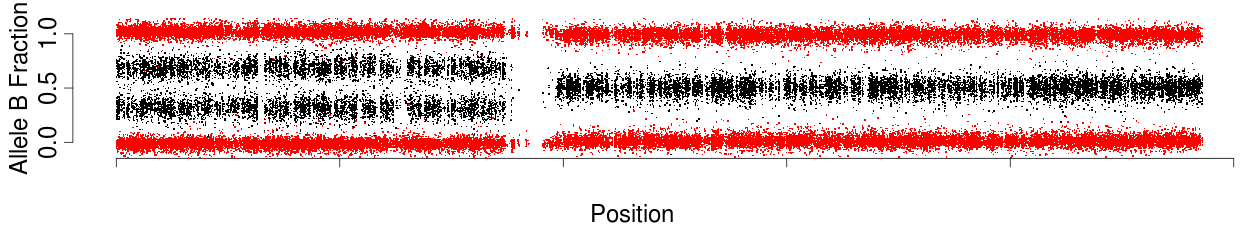
\includegraphics[width=0.8\textwidth]{fig/fracB}\\
					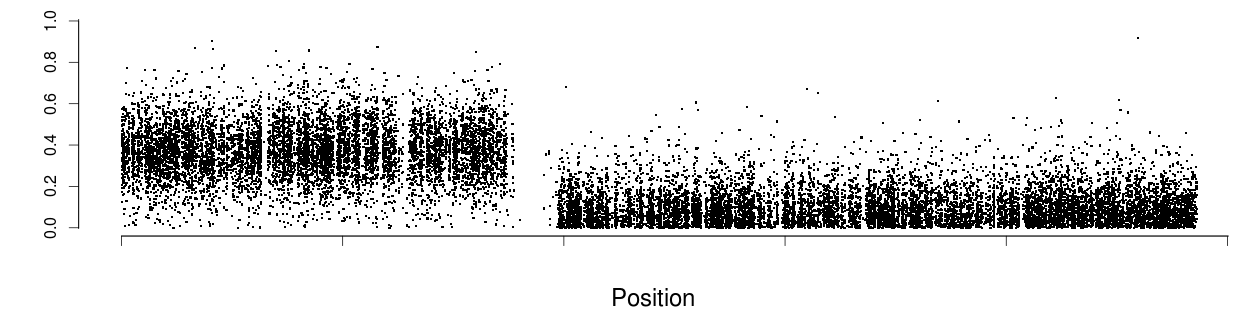
\includegraphics[width=0.8\textwidth]{fig/symFracB}
					\caption{Top: Allele B fraction profile on a chromosome (in red: homozygous SNPs). Bottom: symmetrized profile without homozygous SNPs.}
					\label{figsymFracB}
				\end{figure}

				To perform the segmentation on the allele B fraction, run the following command
\begin{Schunk}
\begin{Sinput}
> #run the segmentation
> segfracB=segFracBSignal("datatest1",chromosome=c(1,5))
> #print summary of segmentation
> segfracB
\end{Sinput}
\end{Schunk}
				 	
		
			\paragraph{Selecting steps to be executed to avoid a complete procedure}

				Each step can be performed with or without the aroma packages if arguments of functions are given in the right format (excepted the normalization procedure described in section \ref{sec:norm}). Almost each wrapper can be used from matrices independently from the other steps and more details are given in the following of this vignette. 
				The paper is organized as follows: the section \ref{sec:norm} presents the preprocessing step and how to access normalized copy-number and allele B fraction. If you already have these data, you can skip this section. Then, an efficient single patient analysis is introduced in the next two sections. The segmentation process is described in section \ref{sec:seg}. In section \ref{sec:calling}, we present the calling process of segmented data. The selection of markers is described in section \ref{sec:select}.


	
\section{Data Normalization}
	\label{sec:norm}

	This preprocessing step consists in a correction of biological and technical biases due to the experiment.
  
  MPAgenomics supports Affymetrix$^{\mbox{\scriptsize{\textregistered}}}$ arrays (5.0, 6.0 and CytoScanHD).	Raw data from Affymetrix DNA chip are provided in different .CEL files. These data need to have some corrections and normalizations before being usable.
  This normalization process can be performed via functions from \texttt{aroma.*} packages \cite{aroma} \cite{affy}. Here, we provide some user-friendly wrappers to these functions.
	We assume that all the required chip files are in the \texttt{chipPATH} folder and the CEL files are in the \texttt{celPATH} folder.
	
	
	\subsection{Folder architecture}\label{arch}
  
		All the functions from aroma packages have to be used with a particular architecture in the working directory. In \texttt{MPAgenomics}, we use the same architecture and provide some functions to create it.

  	A function is provided to create the architecture and copy the specified files in the right directory : \mbox{\texttt{createArchitecture}}. It also checks that the names of the chip files begin by the specified \texttt{chipType} argument.		
		
		\begin{verbatim}
	createArchitecture(dataSetName,chipType,dataSetPath,chipFilesPath,path,verbose,tags)
		\end{verbatim}
	
		\begin{center}
			\begin{tabular}{|l|l|}
				\hline
				Parameters & Description\\
				\hline
				\texttt{dataSetName} & The name of the data-set folder to create.\\
				\texttt{chipType} & The name of the used chip.\\
				\texttt{dataSetPath} &  Path to the folder containing the data CEL files.\\
				\texttt{chipFilesPath} & Path to the folder containing the chip files.\\
				\texttt{path} & Path where the architecture should be created (default=``.'').\\
				\texttt{verbose} & Print information during the process (default=FALSE).\\
        \texttt{tags} & Common tag which appears in the different file names (cdf, ugp, ufl) of the chip. \\
        ~~ & For no tag, use tags=NULL (default = NULL).\\
				\hline	
			\end{tabular}		
		\end{center}
		
		
		For example, assume that we have the downloaded files of the download section (Fig \ref{chipfile} \& \ref{datafileSingle2}).\\
		
		\begin{figure}[!h]
			\centering
			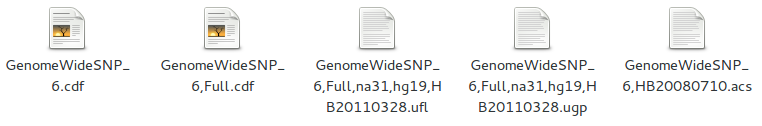
\includegraphics[width=0.6\textwidth]{fig/chipFiles2}\\
			\caption{Chip GenomeWideSNP\_6 files in \texttt{chipPATH} (variable containing the path to the downloaded chip files).}%\texttt{./Documents/chips/SNP6}.}
			\label{chipfile}
		\end{figure}
		
		\begin{figure}[!h]
			\centering
			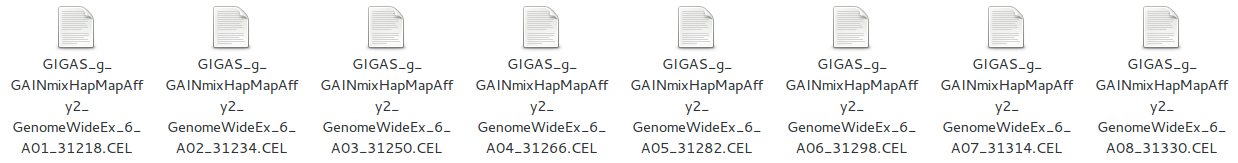
\includegraphics[width=0.9\textwidth]{fig/dataFilesSingle2}
			\caption{CEL files in \texttt{celPATH} (variable containing the path to the downloaded CEL  files).}%\texttt{"./Documents/datatest1"}.}
			\label{datafileSingle2}
		\end{figure}
		
		The \texttt{celPATH} and \texttt{chipPATH} variables contain the different paths to the downloaded files. The following command enables to both create the architecture and add the previous dataset under the name ``datatest1''.
\begin{Schunk}
\begin{Sinput}
> createArchitecture("datatest1","GenomeWideSNP_6",celPATH,chipPATH,".",TRUE,"Full")
\end{Sinput}
\end{Schunk}
		
		
		In your working directory, you must find the following architecture :
		
		\begin{verbatim}
	<current working directory>
  +- annotationData/
  |  +- chipTypes/
  |     +- GenomeWideSNP_6/ 
  |        +- CDF file(s) and other annotation 
  |
  +- rawData/
     +- datatest1/
        +- GenomeWideSNP_6/ 
           +- CEL files
		\end{verbatim}
		
		You can see that files are only copied and not moved.
		~~\\
		This architecture can also be created with the normalization function (see section \ref{norm}).\\
    
    The minimal architecture contains 2 folders: \texttt{annotationData} and \texttt{rawData}. Some supplementary folders will be created during the execution of some functions.

		In the \texttt{annotationData} folder, each type of chip used for the experiment has to have his own folder containing its definition files (.cdf) and other files (.ugp\footnote{See \url{http://www.aroma-project.org/node/43} for more details.}, .acs\footnote{See \url{http://www.aroma-project.org/node/100} for more details.}, .ufl\footnote{See \url{http://www.aroma-project.org/node/47} for more details.}). In this folder, every file name must comply with the following format <chipType>,<tags>.<extension>(see Fig. \ref{chipfile}).
		
		The \texttt{rawData} folder contains the different data-sets with the CEL files. Each data-set folder contains one or more folders (one per different chip type used) containing the CEL files, these files will not be modified during the process. Note that the \texttt{chipType} folder in the data-set folder must match exactly a chip type folder under annotationData.\\
    
    In case of new data-sets or new chip types, it is not useful to create a new architecture but just add new folders in the existing architecture as follows:
		\begin{small}
			\begin{verbatim}
	<current working directory>
  +- annotationData/
  |  +- chipTypes/
  |     +- <chipTypeA>/ <-- must match exactly the name of the CDF file (fullname minus tags)
  |     |  +- CDF file(s) and other annotation (possibly subdirectories)
  |     |
  |     +- <chipTypeB>/ <-- must match exactly the name of the CDF file (fullname minus tags)
  |        +- CDF file(s) and other annotation (possibly subdirectories)
  |        ...
  |
  +- rawData/
  |  +- <dataSet1>/
  |  |  +- <chipTypeA>/ <-- must match exactly a chip type folder under annotationData/
  |  |     +- CEL files
  |  |
  |  +- <dataSet2>/
  |  |  +- <chipTypeB>/ <-- must match exactly a chip type folder under annotationData/
  |  |     +- CEL files
  |  |
  |  +- <dataSet3>/
  |  |  +- <chipTypeA>/ <-- must match exactly a chip type folder under annotationData/
  |  |     +- CEL files
  |  |  +- <chipTypeB>/ <-- must match exactly a chip type folder under annotationData/
  |  |     +- CEL files
  |  ...      
			\end{verbatim}
		\end{small}	
	
		~~\\
		
		In order to easily update your existing architecture you can use the following \texttt{addData} function.
		
		It enables to add to your existing architecture a new data-set in the \texttt{rawData} folder.
		
		\begin{verbatim}
	addData(dataSetName,dataPath,chipType)
		\end{verbatim}
	
		\begin{center}
			\begin{tabular}{|l|l|}
				\hline
				Parameters & Description\\
				\hline
				\texttt{dataSetName} & The name of the data-set folder to create.\\
				\texttt{dataPath} &  Path of the folder containing the data CEL files.\\
				\texttt{chipType} & The name of the used chip.\\ 
				\hline	
			\end{tabular}		
		\end{center}
		
		The \texttt{addChipType} function enables to add to your existing architecture a new chip type in the \texttt{annotationData} folder.
		
		\begin{verbatim}
	addChipType(chipType,chipPath)
		\end{verbatim}
	
		\begin{center}
			\begin{tabular}{|l|l|}
				\hline
				Parameters & Description\\
				\hline
				\texttt{chipType} & Name of the new chip type to add.\\ 
				\texttt{chipPath} & Path to the files to add.\\
				\hline	
			\end{tabular}		
		\end{center}
		
		With the function \texttt{getListOfFiles}, you can obtain the list of the files contained in the specified data-set.
		
		\begin{verbatim}
	getListOfFiles(dataSetName,chipType)
		\end{verbatim}
	
		\begin{center}
			\begin{tabular}{|l|l|}
				\hline
				Parameters & Description\\
				\hline
				\texttt{dataSetName} & The name of a data-set folder.\\
				\texttt{chipType} & The name of the used chip.\\ 
				\hline	
			\end{tabular}		
		\end{center}
		
		If you do not specify a \texttt{chipType}, it returns the files for the first chip in the alphabetic order in the \texttt{dataSetName} folder.
		
		
	\subsection{Normalization process}\label{norm} 
	
		The main function for the normalization of CEL files is \texttt{signalPreProcess}. This function executes 3 different methods on your data:
		\begin{itemize}
			\item \textbf{CRMAv2} \cite{CRMAv2}: Normalize profiles to obtain the copy-number and the allele B fraction. This step consists in the correction of biological and technical biases due to the experiment.
			\item \textbf{Genotype calls}: Assign label $AA$, $AB$ or $BB$ to each SNP.
			\item \textbf{TumorBoost} \cite{TumorBoost}: Only in a case of normal-tumor study, normalization of the allele B fraction tumor profile using the control profile. 
		\end{itemize}
		
		The function \texttt{signalPreProcess} executes all these steps and saves the results in different folders in the aroma architecture (\texttt{totalAndFracBData},\dots), you can also obtain some graphics in the \texttt{figures/signal} folder.
		
		The \texttt{signalPreProcess} is defined as follows:
		\begin{verbatim}	
		signalPreProcess(dataSetName, chipType, normalTumorArray, dataSetPath, chipFilesPath, path,
		createArchitecture, savePlot)
		\end{verbatim}
	
		\begin{center}
			\begin{tabular}{|l|l|}
				\hline
				Parameters & Description\\
				\hline
				\texttt{dataSetName} & The name of the data-set.\\
				\texttt{chipType} & The type of the used chip (e.g. ``GenomeWideSNP\_6'').\\
				\texttt{normalTumorArray} & Only in the case of normal-tumor study. A csv file or a data.frame\\
				~~ & containing the mapping between normal and tumor files(Fig. \ref{normalTumorArray}).\\
				\texttt{dataSetPath} & Only if \texttt{createArchitecture=TRUE}.\\
				~~ & Path to the folder containing the CEL files of the data-set.\\
				\texttt{chipFilesPath} & Only if \texttt{createArchitecture=TRUE}.\\
				~~ & Path to the folder containing all the annotations files for the specified chip type.\\
				\texttt{path} & Only if \texttt{createArchitecture=TRUE}.\\
				~~ & Path where the architecture should be created (default=``.'').\\
				\texttt{createArchitecture} & if TRUE, the aroma architecture will be automatically created (default=TRUE).\\
				\texttt{savePlot} & if TRUE, graphics of the CN signal and allele B fraction signal will be\\
				~~ & saved in the \texttt{figures/signal} folder. (default=TRUE).\\
        \texttt{tags} & Common tag which appears in the different filenames (cdf, ugp, ufl) of the chip. \\
        ~~ & For no tag, use tags=NULL (default = NULL).\\
				\hline	
			\end{tabular}		
		\end{center}
	
		\begin{figure}[!h]
			\centering
			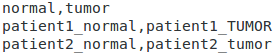
\includegraphics[width=0.3\textwidth]{fig/normalTumorArray}\\
			\caption{Example of the content of a csv file for \texttt{normalTumorArray} parameter. The first column contains the name of the different normal files (without the .cel extension) in the data-set folder in rawData. The second column contains the name of the tumor files. The name of the two columns are respectively normal and tumor. The extensions of the files (.CEL for example) should be removed.}
			\label{normalTumorArray}
		\end{figure}

		If you have specified \texttt{createArchitecture=TRUE} and have given the required parameters, the function will create the architecture and copy your files in the right folder. After the creation of the aroma architecture, it runs the normalization process and saves in the aroma architecture all the files necessary to obtain the allele B fraction and the copy-number signal.\\
		
		In the case of a study without reference, only parameters \texttt{dataSetName}, \texttt{chipType}, \texttt{createArchitecture} and \texttt{savePlot} have to be specified. In the case of a normal-tumor study, TumorBoost process is executed.
		If you want a CEL file to be used as reference for all the tumor data, then fill the normal column of the \texttt{normalTumorArray} with the filename of your reference for all files.
		
	\subsection{Accessing the copy-number,  allele B fraction and genotype}		
		\label{getter}
		After running the \texttt{signalPreProcess} function, you can not directly access the copy-number and the allele B fraction signals with the files in the architecture, a treatment is required to read them. Note that the copy-number signal saved is the raw signal, it needs a reference to normalize it. With the \texttt{getCopyNumberSignal} and \texttt{getFracBSignal} functions, you can access the copy-number and the allele B fraction profiles.\\
		
		The \texttt{getCopyNumberSignal} allows you to extract the copy-number signal a chromosome at a time. In the case of a study without reference, the median of all the signals of the data-set is used to normalize every profile. In the normal-tumor study, the normal signal is used to normalize the tumor signal.
		
		The getter for the copy-number profile is defined as follows:
		\begin{verbatim}	
		getCopyNumberSignal(dataSetName,chromosome,normalTumorArray,onlySNP,listOfFiles,verbose)
		\end{verbatim}
	
		\begin{center}
			\begin{tabular}{|l|l|}
				\hline
				Parameters & Description\\
				\hline
				\texttt{dataSetName} & The name of the data-set folder.\\
				\texttt{chromosome} & A vector containing the chromosomes for which the signal will be extracted.\\
				\texttt{normalTumorArray} & Only in the case of normal-tumor study. A csv file or a data.frame\\
				~~ & containing the mapping between normal and tumor files(Fig. \ref{normalTumorArray}).\\
				\texttt{onlySNP} & If TRUE, only the copy-number for SNPs positions will be returned (default=FALSE).\\
				\texttt{listOfFiles} & A vector containing the names of the files in dataSetName folder for which\\
				~ & the copy-number profiles will be extracted (default is all the files).\\
				\texttt{verbose} & If TRUE print some information (default=TRUE).\\
				\hline	
			\end{tabular}		
		\end{center}
		
		This function returns a list of size \texttt{length(chromosome)} (each element is named \texttt{chrX} with \texttt{X} the number of the chromosome) containing a data.frame with columns:
		\begin{itemize}
			\item \textbf{chromosome} Chromosome of the signal.
			\item \textbf{position} Positions associated with the copy-number.
			\item \textbf{copynumber} Copy number profiles of selected files; the name of each column is the name of the associated data file name. 			
			\item \textbf{featureNames} Names of the probes.
		\end{itemize}
		~~\\
		
		If you want the allele B fraction, you can use the \texttt{getFracBSignal} function. In a normal-tumor study, allele B fraction for both normal and tumoral samples is returned. For the tumoral sample, it is the allele B fraction after the TumorBoost normalization.
		
		\begin{verbatim}	
		getFracBSignal(dataSetName,chromosome,normalTumorArray,listOfFiles,verbose)
		\end{verbatim}
	
		\begin{center}
			\begin{tabular}{|l|l|}
				\hline
				Parameters & Description\\
				\hline
				\texttt{dataSetName} & The name of the data-set folder.\\
				\texttt{chromosome} & A vector containing the chromosomes for which the allele B fraction signal must be extract.\\
				\texttt{normalTumorArray} & Only in the case of normal-tumor study. A csv file or a data.frame\\
				~~ & containing the mapping between normal and tumor files(Fig. \ref{normalTumorArray}).\\
				\texttt{listOfFiles} & A vector containing the names of the files in dataSetName folder for which\\
  			~ & the allele B fraction profiles will be extracted (default is all the files).\\
				\texttt{verbose} & If TRUE print some information (default=TRUE).\\
				\hline	
			\end{tabular}		
		\end{center}
				

		This function returns a list of size \texttt{length(chromosome)} (each element is named \texttt{chrX} with \texttt{X} the number of the chromosome) containing a data.frame with columns:
		\begin{itemize}
			\item \textbf{chromosome} Chromosome of the signal.
			\item \textbf{position} Positions associated with the allele B fraction.
			\item \textbf{fracB} Allele B fraction profiles of selected files; the name of each column is the name of the associated data file name. 		
			\item \textbf{featureNames} Names of the probes.
		\end{itemize}
		~~\\
		
		If you want the genotype call, you can use the \texttt{getGenotypeCalls} function. 
		
		\begin{verbatim}	
		getGenotypeCalls(dataSetName,chromosome,listOfFiles=NULL,verbose=TRUE)
		\end{verbatim}
	
		\begin{center}
			\begin{tabular}{|l|l|}
				\hline
				Parameters & Description\\
				\hline
				\texttt{dataSetName} & The name of the data-set folder.\\
				\texttt{chromosome} &  A vector containing the chromosomes for which the genotype call will be extracted.\\
				\texttt{listOfFiles} & A vector containing the names of the files in dataSetName folder for which\\
				~ & the genotype signal will be extracted (default is all the files).\\
				\texttt{verbose} & If TRUE print some information (default=TRUE).\\
				\hline	
			\end{tabular}		
		\end{center}
				
		This function returns a list of size \texttt{length(chromosome)} (each element is named \texttt{chrX} with \texttt{X} the number of the chromosome) containing a data.frame with columns:
		\begin{itemize}
			\item \textbf{chromosome} Chromosome of the signal.
			\item \textbf{position} Positions associated with the genotype.
			\item \textbf{genotype} Genotype calls corresponding to selected files; the name of each column is the name of the associated data file name. 
			\item \textbf{featureNames} Names of the probes.
		\end{itemize}
		
		
		~~\\
		The next getter, \texttt{getSymFracBSignal}, returns the symmetrized allele B fraction only for heterozygous positions. To symmetrize the allele B fraction the transformation $x\mapsto 2*|x-0.5|$ is applied. It centers the data in $0.5$ corresponding to heterozygous allele B fraction then symmetrize and multiply by $2$ to have a signal between $0$ and $1$. \\
    
    This method can be run only in a normal-tumor case, and each tumor file must match with a unique normal file.
		
		\begin{verbatim}	
		getSymFracBSignal(dataSetName,chromosome,normalTumorArray,file,verbose=TRUE)
		\end{verbatim}
	
		\begin{center}
			\begin{tabular}{|l|l|}
				\hline
				Parameters & Description\\
				\hline
				\texttt{dataSetName} & The name of the data-set folder.\\
				\texttt{chromosome} & A vector with the chromosomes for which the symetrized signal will be extracted .\\
				\texttt{normalTumorArray} & A csv file or a data.frame \\
				~~ & containing the mapping between normal and tumor files(Fig. \ref{normalTumorArray}).\\
				\texttt{file} & The name of the file in dataSetName folder for which\\
				~ & the symetrized signal will be extracted .\\
				\texttt{verbose} & If TRUE print some information (default=TRUE).\\
				\hline	
			\end{tabular}		
		\end{center}
				
		This function returns a list of size \texttt{length(chromosome)} (each element is named \texttt{chrX} with \texttt{X} the number of the chromosome) containing a data.frame with columns:
		\begin{itemize}
			\item \textbf{chromosome} Chromosome of the signal.
			\item \textbf{position} Positions associated with the genotype.
			\item \textbf{fracB} One column named by the data file name. It contains the symmetrized allele B fraction signal for the specified profile.			
			\item \textbf{featureNames} Names of the probes.
		\end{itemize}
		
		
	\subsection{Usage}
	
  We refer to sections \ref{mainuse} and \ref{mainusecontrol} to normalize input data without or with control samples in the study, respectively.	

\paragraph*{Get a signal}~~\\
		The following commands enable to extract the copy-number or the allele B fraction profiles of all the files for the chromosome 5:
		
\begin{Schunk}
\begin{Sinput}
> #normal-tumor study
> CNdata2=getCopyNumberSignal("datatest2",5,normalTumorArray=normalTumorArray,TRUE)
> fracBdata2=getFracBSignal("datatest2",5,normalTumorArray=normalTumorArray)
> #study without reference
> CNdata1=getCopyNumberSignal("datatest1",5,onlySNP=TRUE)	
> fracBdata1=getFracBSignal("datatest1",5)		
\end{Sinput}
\end{Schunk}
		
		To access the copy-number or allele B fraction profiles, run:
\begin{Schunk}
\begin{Sinput}
> CNdata2$chr5
> fracBdata2$chr5$tumor
> fracBdata2$chr5$normal
> fracBdata1$chr5$tumor
\end{Sinput}
\end{Schunk}
				


\section{Segmentation}
	\label{sec:seg}
	
	In the package \texttt{MPAgenomics}, we provide two segmentation methods.
  The first one wraps the \texttt{cghseg} package which fits a Gaussian maximum-likelihood piecewise constant smoothing model \cite{cghsegb} using pruned dynamic programming \cite{cghseg}. When the user chooses this method, \texttt{MPAgenomics} selects the number of segments with the slope heuristic \cite{heurpente}. 
  
  The second segmentation approach uses the PELT method of the \texttt{cpt.mean} function from the \texttt{changepoint} package \cite{peltR}.
	In the initial PELT method, the penalty is $K\rho\log(P)$ with a profile of length $P$, $K$ the number of segments and a $\rho>0$ a constant to optimize. When the user chooses this method, \texttt{MPAgenomics} suggests another calibration for the penalty parameter. For more details, see Section \ref{sec:togo}.
  
	
	\subsection{From data normalized by aroma}	
		
		The procedure described above can be run by the \texttt{segmentationAroma} function if the working directory respects the aroma architecture.
		 	
		\begin{verbatim}	
segmentationAroma(dataSetName,normalTumorArray,chromosome,Rho=NULL,Kmax=10,listOfFiles=NULL,onlySNP=TRUE,
savePlot=TRUE,method="cghseg")
		\end{verbatim}
	
		\begin{center}
			\begin{tabular}{|l|l|}
				\hline
				Parameters & Description\\
				\hline
				\texttt{dataSetName} & The name of the data-set folder.\\
				\texttt{normalTumorArray} & Only in the case of normal-tumor study. A csv file or a data.frame\\
				~~ & containing the mapping between normal and tumor files(Fig. \ref{normalTumorArray}).\\
				\texttt{chromosome} & A vector with the chromosomes to be segmented.\\
				\texttt{Rho} & Only for method=``PELT'', a vector containing all the penalization values to test \\
				~ &  for the segmentation. If no values are provided, default values will be used.\\
        \texttt{Kmax} & Only for method=``cghseg'', maximal number of segments.\\
				\texttt{onlySNP} & If TRUE, only the copy-number for SNPs positions will be returned (default=TRUE).\\
				\texttt{listOfFiles} & A vector containing the names of the files in dataSetName folder for which\\
				~ & the copy number profiles  will be segmented (default is all the files).\\
				\texttt{savePlot} & if TRUE, graphics of the segmented CN signal will be\\
				~~ & saved in the \texttt{figures/dataSetName/segmentation/CN} folder. (default=TRUE).\\
				\texttt{method} & ``PELT'' or ``cghseg''. (default=``PELT'').\\
				\hline
			\end{tabular}		
		\end{center}
	
			If \texttt{savePlot=TRUE}, some graphics will be plotted (see Fig \ref{outpelt}).\\
	
		\begin{figure}[!h]
			\centering
			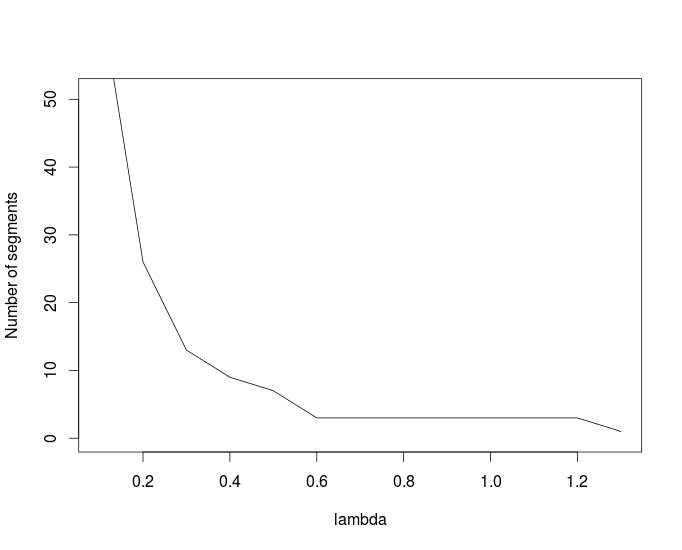
\includegraphics[width=0.45\textwidth]{fig/decdata1}
			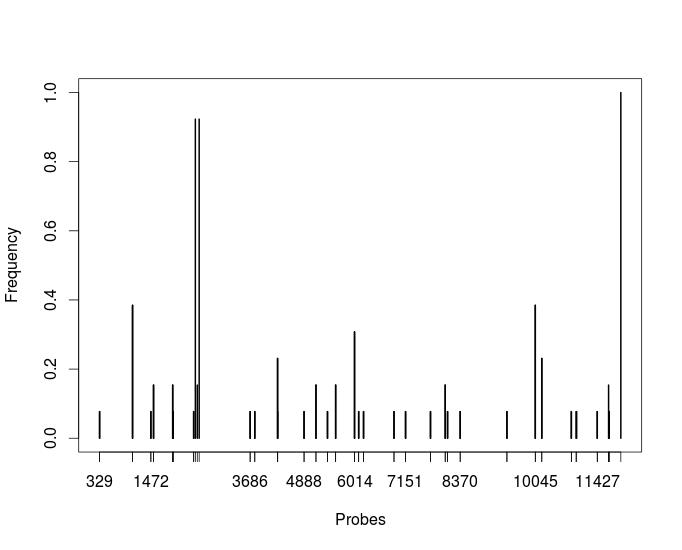
\includegraphics[width=0.45\textwidth]{fig/freqdata1}\\		
			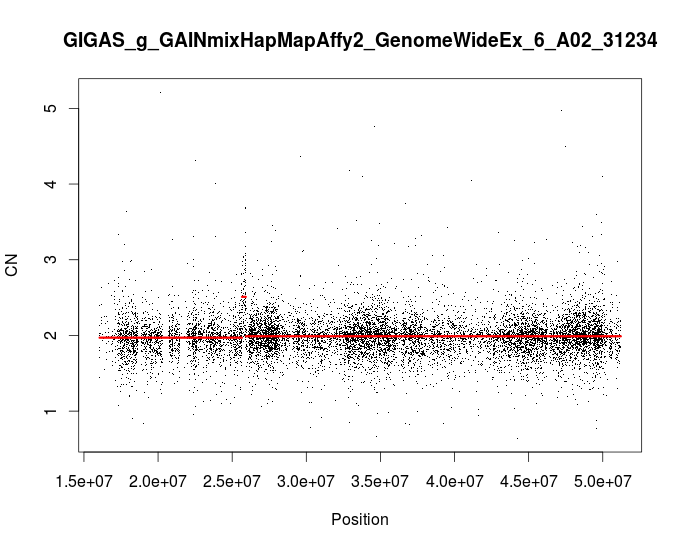
\includegraphics[width=0.5\textwidth]{fig/segdata1}
			\caption{Top left: variation of the number of segments with regards to $\rho$. Top right: the frequency of occurrence of breakpoints in all segmentation. Bottom: Segmentation with the optimal $\rho$ found.}
			\label{outpelt}
		\end{figure}
		The graphics of the segmented profiles are saved in the \texttt{figures/dataSetName/segmentation} folder. A summary of the segmented profile is saved in a text file (Fig. \ref{outbedpelt}) in the \texttt{segmentation/dataSetName/} folder, it contains 5 columns: chrom, chromStart, chromEnd, probes and means containing the number of the chromosome, the starting position of the segment, the ending position of the segment, the number of probes in the segment and the mean of the segment.\\
	
		\begin{figure}[!h]
			\centering
			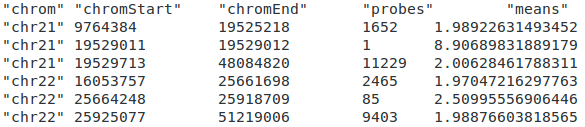
\includegraphics[width=0.4\textwidth]{fig/outbedpelt}
			\caption{Summary of a segmentation for a profile.}
			\label{outbedpelt}
		\end{figure}
		
		The output of the function is a list where every element of the list contains the segmentation results for a different profile formatted in a list containing:
		\begin{itemize}
			\item \textbf{copynumber} A vector containing  the copy-number signal.
			\item \textbf{segmented} A vector of the same size as copynumber containing the segmented values.
			\item \textbf{startPos} The position of every probe.
			\item \textbf{chromosome} A vector of the same size as copynumber containing the chromosome number.
			\item \textbf{featureNames} Names of the probes.
			\item \textbf{sampleNames} The name of the signal.
			\item \textbf{segment} A data.frame that sums up the results of the segmentation. Each row is a different segment with the chromosome, start position, end position, number of probes in the segment and the value of the segment.
		\end{itemize}
				
		The output for a profile is formatted in order to be usable in input of the \texttt{callingProcess} function (see section \ref{calling}) but if you use the aroma architecture and want to label your segments, you can directly use the \texttt{cnSegCallingProcess} function (see section \ref{segcalling}). This function runs the segmentation and the calling processing.
		
		~~\\
		
		In the following example, the segmentation processing is run on one file of the downloaded data:
		
\begin{Schunk}
\begin{Sinput}
> file="GIGAS_g_GAINmixHapMapAffy2_GenomeWideEx_6_A02_31234"
> seg1=segmentationAroma("datatest1",chromosome=21:22,onlySNP=TRUE,plot=TRUE,
+ listOfFiles=file,method="PELT")
\end{Sinput}
\end{Schunk}
		
		The results obtained for one profile are shown in figures \ref{outpelt} \& \ref{outbedpelt}.
		
		~~\\
	  
		For a normal-tumor study where each tumor file matches with a unique normal file (and only in this case), it is possible to segment the symmetrized allele B fraction with the function \texttt{segFracBSignal}:
		 	
		\begin{verbatim}	
segFracBSignal(dataSetName,normalTumorArray,chromosome=1:22,Rho=NULL,Kmax=10,listOfFiles=NULL,
savePlot=TRUE,verbose=TRUE,method="cghseg")
		\end{verbatim}
	
		\begin{center}
			\begin{tabular}{|l|l|}
				\hline
				Parameters & Description\\
				\hline
				\texttt{dataSetName} & The name of the data-set folder.\\
				\texttt{normalTumorArray} & A csv file or a data.frame\\
				~~ & containing the mapping between normal and tumor files(Fig. \ref{normalTumorArray}).\\
				\texttt{chromosome} & A vector with the chromosomes to be segmented.\\
  			\texttt{Rho} & Only for method=``PELT'', a vector containing all the penalization values to test\\
				~ &  for the segmentation. If no values are provided, default values will be used.\\
        \texttt{Kmax} & Only for method=``cghseg'', maximal number of segments.\\
				\texttt{listOfFiles} & A vector containing the names of the files in dataSetName folder for which\\
				~ & the allele B profile is segmented (default is all the files).\\
				\texttt{savePlot} & if TRUE, graphics of the segmented allele B profile will be\\
				~~ & saved in the \texttt{figures/dataSetName/segmentation/fracB} folder. (default=TRUE).\\
        \texttt{verbose} & If TRUE, print some information (default=TRUE).\\
				\hline	
			\end{tabular}		
		\end{center}		
		
			
		The output of the function is a data.frame containing the segmentation results, each row corresponding to a different segment and with columns:
		\begin{itemize}
			\item \textbf{sampleName} Name of the file the segment belongs to.
			\item \textbf{chromosome} Chromosome the segment belongs to.
			\item \textbf{chromStart} Starting position of the segment.
			\item \textbf{chromEnd} Ending position of the segment.
			\item \textbf{probes} Number of probes in the segment.
			\item \textbf{means} Mean of the segment.
		\end{itemize}
			
	\subsection{For any data provided in matrices}	
		Assuming that normalized data are stored in a matrix, you can use the \texttt{segmentation} function to perform segmentations with parameter choices suggested in \texttt{MPAgenomics}.
	
		\begin{verbatim}	
			segmentation(signal,Rho=NULL,Kmax=10,position=NULL,plot=TRUE,verbose=TRUE,method="cghseg")
		\end{verbatim}
	
		\begin{center}
			\begin{tabular}{|l|l|}
				\hline
				Parameters & Description\\
				\hline
				\texttt{signal} & A vector containing the signal.\\
    		\texttt{Rho} & Only for method=``PELT'', a vector containing all the penalization values to test\\
				~ & for the segmentation. If no values are provided, default values will be used.\\
        \texttt{Kmax} & Only for method=``cghseg'', maximal number of segments.\\
				\texttt{position} & A vector containing the position of all elements of the signal (not necessary).\\
				\texttt{plot} & If TRUE, plot some graphics (default=TRUE	).\\
				\texttt{verbose} & If TRUE, print some information (default=TRUE).\\
        \texttt{method} & ``PELT'' or ``cghseg''. (default=``PELT'').\\
				\hline	
			\end{tabular}		
		\end{center}
		
		If \texttt{plot=TRUE}, some graphics will be plotted (see Fig \ref{outpelt}).
	
		
		The output of the function is a list containing:
		\begin{itemize}
			\item \textbf{signal} A vector containing the signal.
			\item \textbf{segmented} A vector of the same size as the signal containing the segmented values.
			\item \textbf{startPos} The position of each probe.
			\item \textbf{segment} A data.frame that sums up the results of the segmentation. Each row is a different segment with the start position, end position, number of points in the segment and the value of the segment.
		\end{itemize}

%		This output can be used directly in argument of the calling function \texttt{callingProcess} (see section \ref{calling}).
		~~\\
	
		For the following example, a matrix is built from the preprocessed files obtained in section \ref{norm}. A copy number profile from one patient chromosome is then isolated: 
	
\begin{Schunk}
\begin{Sinput}
> file="GIGAS_g_GAINmixHapMapAffy2_GenomeWideEx_6_A07_31314"
> CNdata1=getCopyNumberSignal("datatest1",20,onlySNP=TRUE,listOfFiles=file)
> copyNumber=CNdata1$chr20$GIGAS_g_GAINmixHapMapAffy2_GenomeWideEx_6_A07_31314
> position=CNdata$chr20$position
\end{Sinput}
\end{Schunk}
	
		Then, the segmentation process can be run using:
\begin{Schunk}
\begin{Sinput}
> seg=segmentation(copyNumber,position=position,plot=TRUE,verbose=TRUE,method="PELT")
\end{Sinput}
\end{Schunk}
	
		This leads to the same plots as in Fig \ref{outpelt} and the results are saved in the right format for the calling function (see section \ref{calling}).
	
		The list of found segments can be accessed with: 
\begin{Schunk}
\begin{Sinput}
> seg$segment
\end{Sinput}
\end{Schunk}
	
		\begin{figure}[!h]
			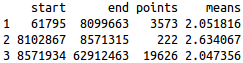
\includegraphics[width=0.3\textwidth]{fig/outpelt2}
		\end{figure}
		
		
    \subsection{To go further}
      \label{sec:togo}
        In this part, we describe the different calibration methods associated with cghseg and PELT in \texttt{MPAgenomics}. We also illustrate that calibrating the parameter according to a variance criterium can be misleading.
        
  
      \subsubsection{Choice of the number of segments for cghseg}
        cghseg method runs with a predetermined number of segments. In general, users fix a maximal number of segments $K_{\max}$ and then must choose the best segmentation according to some criteria. \texttt{MPAgenomics} implements the slope heuristic \cite{heurpente} to choose automatically the number of segments. 
      
        Let $k$ the number of segments, the criterium \cite{penseg} to minimize is 
        $$g(k,C)=\frac{1}{P}\left(R(k)+C\times k \times \left(2.5+\log(\frac{P}{k})\right)\right) $$
      
        where $R(k)$ is the quadratic loss between the observed and the segmented signal, and $C$ a constant to optimize.
      
        The first step is to find the optimal constant $\hat{C}$ to use. Given a list $\mathcal{C}$ of potential constant, for each element $C\in\mathcal{C}$, we find the optimal $\hat{k}$ minimizing $g(k,C)$. Then, the optimal constant $\hat{C}$ is $2\times C_0$, whith $C_0$ the constant associated with the largest drop of the number of segments in Fig. \ref{fig:slopeheuristic}.  
      
        \begin{figure}[!h]
          \centering
  	      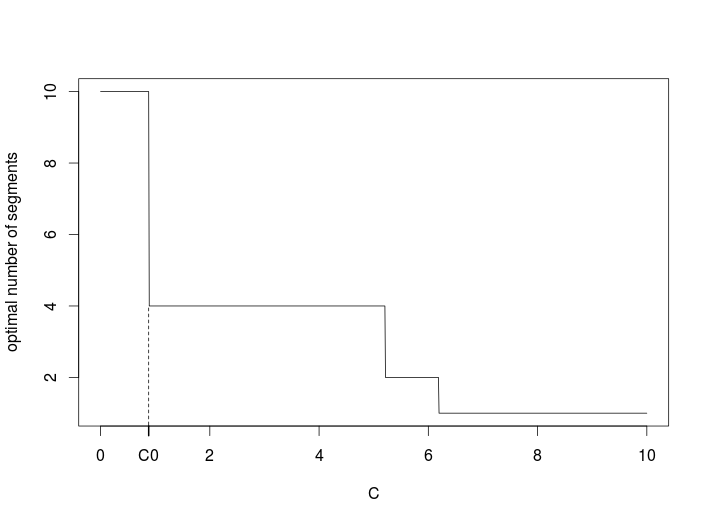
\includegraphics[width=0.5\textwidth]{fig/slopeheuristic}
		      \caption{Optimal number of segments minimizing $g(C,k)$ with regards to $C$. $C_0$ is the constant associated with the largest drop of the number of segments.}
		      \label{fig:slopeheuristic}
        \end{figure}
      
        Once the optimal constant $\hat{C}$ found, the optimal number of segments $\hat{k}$ is the one minimizing $g(k,\hat{C})$.
      
      
      \subsubsection{Choice of the number of segments for PELT}
        \label{sec:calib}
        The penalty of PELT looks like $\rho\times K \times\log(P)$ with $K$ the number of segments and $P$ the length of the profile. Only the parameter $\rho$ can be chosen by the user.
        As the default value in PELT ($\rho=1$) did not provide satisfying segments compared to manually annotated segments, which we observed on 70 profiles, we suggest another method to calibrate the $\rho$ parameter.
        To make the choice of the optimal $\rho$ in \texttt{MPAgenomics}, the PELT method is run for a range of $\rho$ provided by default or given by the user. Then, the evolution of the number of segments is plotted with regards to the $\rho$ parameter (Fig \ref{plateau}). 
  
        \begin{figure}[!h]
		      \centering
		      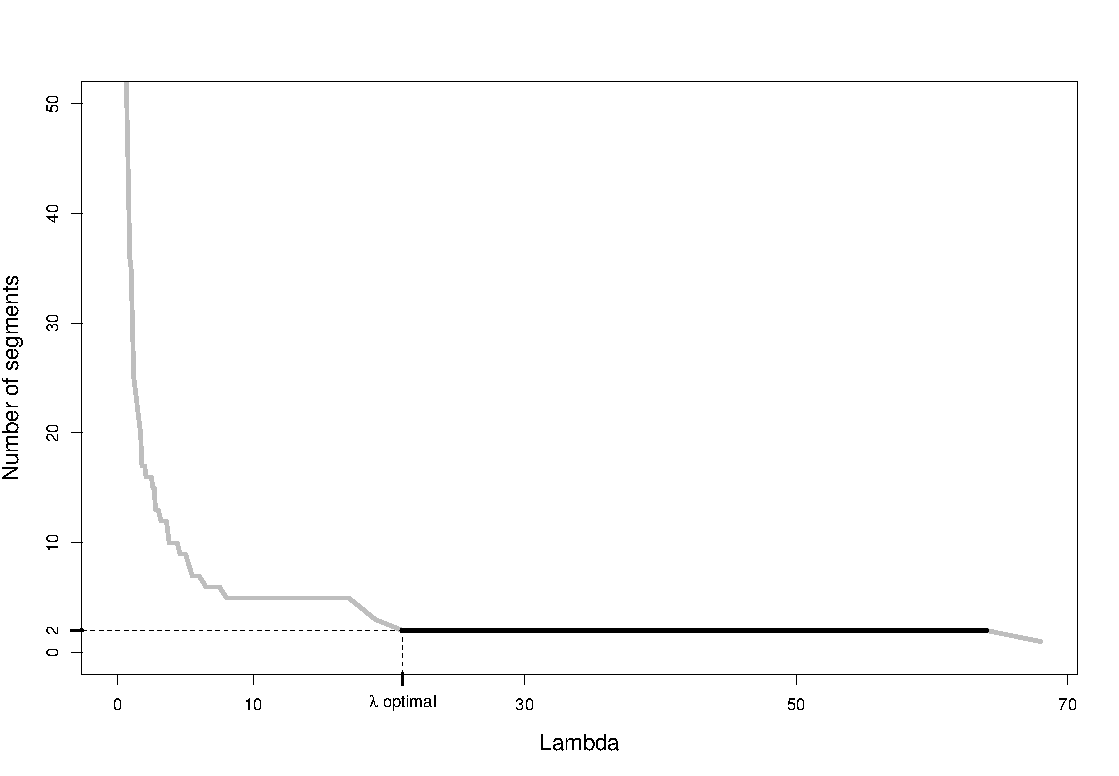
\includegraphics[width=0.5\textwidth]{fig/plateau}
		      \caption{Variation of the number of segment with regards to rho.}
		      \label{plateau}
	      \end{figure}
	
        We want to adjust the $\rho$ parameter to have a reasonable number of segments. So, we look for the widest range of $\rho$ for which the number of segments remains unchanged (and larger than 1). Indeed, our intuition is that we can be confident in the found breakpoints because the penalty has to increase significantly to remove some breakpoints. The optimal data-driven $\rho$ is the left-most value of the widest range such that the number of segments is larger than 1. Otherwise we consider there is only one segment in the profile.
          
        \paragraph*{Sample-specific versus common parameter}
      
          The \textit{sample-specific choice of $\rho$} described above was empirically compared with a \textit{common choice of  $\rho$} depending on the signal-to-noise ratio within each group of given profiles.
          Seventy profiles from a real dataset \cite{citerealdataset} were clustered into groups with homogeneous signal-to-noise ratio (SNR) by using a Gaussian mixture model. Three groups were provided by the BIC criterion. 

          Figure~\ref{fig:classifplateau} displays results (chromosome~1) for each profile (patient). Following Section~\ref{sec:calib} the widest range of $\rho$ values was plotted for each profile. 
          Colors (light grey, grey, and black) indicate the SNR level in each group (respectively low, middle, and high).
	
          \begin{figure}[!h]
	          \centering
	          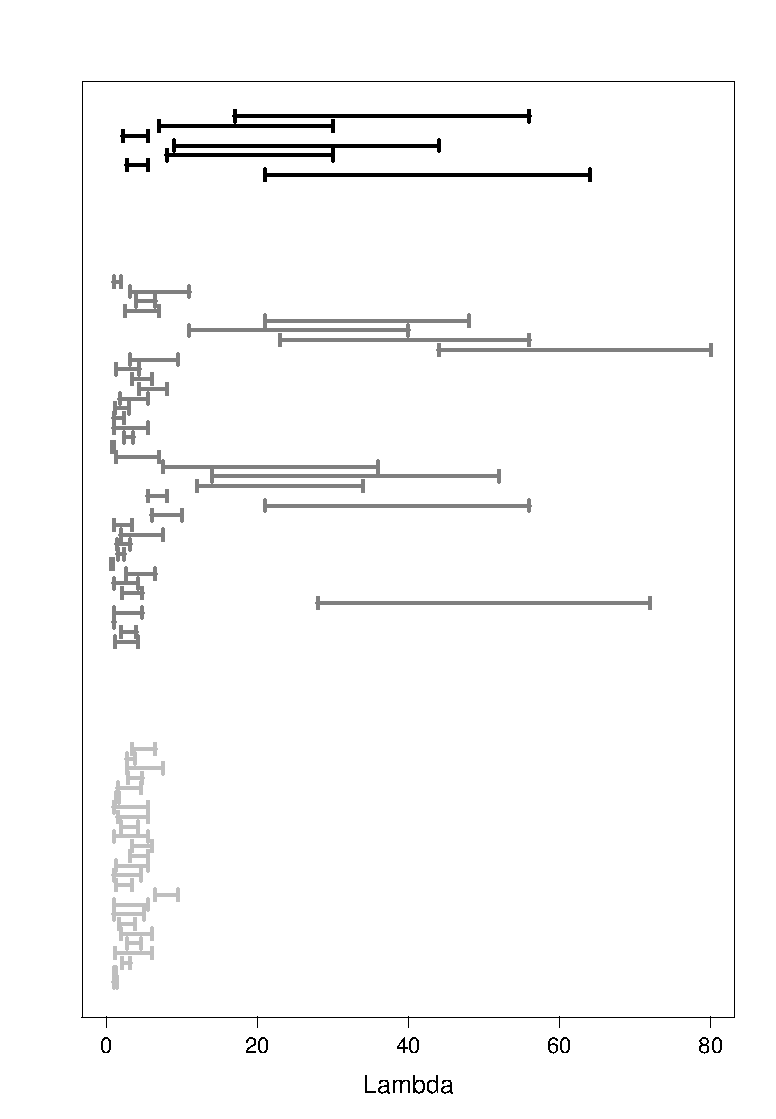
\includegraphics[width=0.4\textwidth]{fig/classifplateau3}
            \caption{Widest ranges of $\rho$ ($x$-axis) for 70 copy number profiles (chromosome 1) ($y$-axis). Colors indicate clusters of signal-to-noise ratios (light grey $<$ grey $<$ black).}
            \label{fig:classifplateau}
          \end{figure}

          Whereas the lowest SNR group only contains ranges of $\rho$ with small values, other groups correspond to ranges of both small and large values of $\rho$. A common choice of $\rho$ within each of these two groups would have led to erroneous segmentations. The same conclusion applied to other chromosomes and criteria such as variance. 

	
\section{Calling aberrations in copy-number profiles}
	\label{sec:calling}
  
  When performing segmentations with cghseg or PELT, labels of segments ($loss$, $normal$ or $gain$) are not known. It is possible to assign these labels with the \texttt{CGHcall} method \cite{CGHcall}. A wrapper of the CGHcall calling process is available in \texttt{MPAgenomics}.
	
	Starting with a signal and an associated segmented profile, the method assumes that the segmented values follow a mixture of Gaussians. The parameters of the model are estimated with an EM algorithm with a specific initialization. Then, every segment is called by the most likely label according to the modeL. 
	
	\subsection{From data normalized by aroma}	
		\label{segcalling}
		The \texttt{cnSegCallingProcess} function executes the segmentation (see section \ref{sec:seg}) and the calling process. The specified data will be automatically imported by the function.\\
			
		\begin{verbatim}	
		cnSegCallingProcess(dataSetName,normalTumorArray,chromosome,Rho,Kmax,listOfFile,onlySNP,savePlot,
		nclass,cellularity,method,...)
		\end{verbatim}
		
		\begin{tabular}{|l|l|}
			\hline
			Parameters & Details\\
			\hline
			\texttt{dataSetName} & name of the data-set folder in the rawData folder containing the signals to use.\\
			\texttt{normalTumorArray} & Only in the case of normal-tumor study. A csv file or a data.frame\\
			~ & containing the mapping between normal and tumor files(Fig. \ref{normalTumorArray}).\\
			\texttt{chromosome} & A vector containing the chromosome to segment.\\
  		\texttt{Rho} & Only for method=``PELT'', a vector containing all the penalization values to test \\
			~ &  for the segmentation. If no values are provided, default values will be used.\\
      \texttt{Kmax} & Only for method=``cghseg'', maximal number of segments.\\
			\texttt{listOfFiles} & A vector containing the file names from the dataSetName to use.\\
			\texttt{onlySNP} & If TRUE, only the SNP probes will be used.\\
			\texttt{savePlot} & If TRUE, print some graphics (default=TRUE).\\
			\texttt{nclass} & The number of levels to be used for calling. Either 3 (loss, normal, gain),\\
			~ &   4 (including amplifications), 5 (including double deletions) (default=3).\\
			\texttt{cellularity} &  Percentage of tumor cells in the sample (default=1).\\
			\texttt{\dots} & Other parameters for the CGHcall function \cite{CGHcallR}.\\
      \texttt{method} & ``PELT'' or ``cghseg''. (default=``PELT'').\\
			\hline
		\end{tabular}

~~\\

		This function will save every segment in a text file in the \texttt{segmentation} folder in the working directory and return a data.frame with columns:
			
		\begin{itemize}
			\item \textbf{sampleNames} Name of the file.
			\item \textbf{chrom} The chromosome of the segment.
			\item \textbf{chromStart} The starting position (in bp) of the segment. This position is not included in the segment.
			\item \textbf{chromEnd} The ending position (in bp) of the segment. This position is included in the segment.
			\item \textbf{probes} Number of probes in the segment.
			\item \textbf{means} Mean of the segment.
			\item \textbf{calls} The calling of the segment (``double loss'', ``loss'', ``normal'', ``gain'' or ``amplification'').
		\end{itemize}
			
		The graphic of the segmented profile is saved in the \texttt{figures} folder of the architecture.
			
\begin{Schunk}
\begin{Sinput}
> seg2=cnSegCallingProcess("datatest1",chromosome=21:22,method="PELT")
\end{Sinput}
\end{Schunk}
			
		The output of the function is shown in the figure \ref{segcalloutput}.
		\begin{figure}[!h]
			\centering
			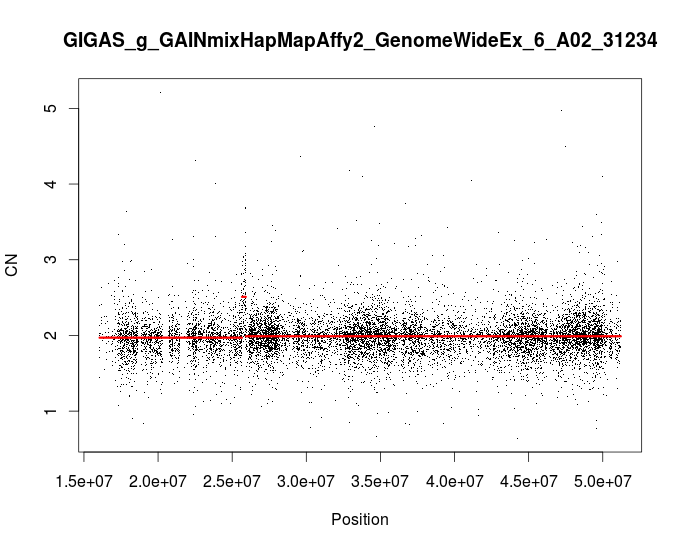
\includegraphics[width=0.5\textwidth]{fig/segdata1}
			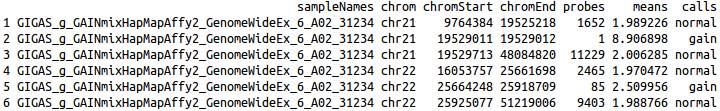
\includegraphics[width=0.5\textwidth]{fig/callsoutput}
			\caption{Top: graphics saved in the \texttt{figures} folder. Bottom: output of the function (saved in a text file too).}
			\label{segcalloutput}
		\end{figure}
	
	
	\subsection{For any data provided in matrices}\label{calling}
	
		The function \texttt{callingProcess} executes all the calling process and can be used without the aroma architecture. You can use this function with the segmentation method provided in the package or any other methods as long as you give the results of the segmentation in the right format (see \texttt{segmentData} argument).
	
		\begin{verbatim}	
		callingProcess(segmentData,nclass=5,cellularity=1,...)
		\end{verbatim}
	
		\begin{center}
			\begin{tabular}{|l|l|}
				\hline
				Parameters & Description\\
				\hline
				\texttt{segmentData} & A list (see details below).\\
				\texttt{nclass} & Number of labels. 3 corresponds to ``loss'', ``normal'' and ``gain'', \\
				~ & 4 adds ``amplification'' and 5 adds ``double loss''.\\
				\texttt{cellularity} & Percentage of tumor cells in the sample (default=1).\\
				\texttt{verbose} & If TRUE, print some information.\\
				\texttt{\dots} & Others parameters for CGHcall function \cite{CGHcallR}.\\
				\hline	
			\end{tabular}		
		\end{center}
		
	
		
		\texttt{segmentData} is a list containing:
		\begin{itemize}
			\item \textbf{copynumber} A matrix. Every column represents a copy-number signal for a different sample.
			\item \textbf{segmented} A matrix of the same size as \texttt{copynumber} containing the segmented values of the copy-number signal.
			\item \textbf{chromosome} A vector, of length the number of rows of \texttt{copynumber} matrix, containing the number of the chromosome for each position.
			\item \textbf{startPos} A vector, of length the number of rows of \texttt{copynumber} matrix, containing the genomic position of each probe.
			\item \textbf{featureNames} A vector, of length the number of rows of \texttt{copynumber} matrix, containing the name of each probe.
			\item \textbf{sampleNames} A vector, of length the number of columns of \texttt{copynumber} matrix, containing the name of each file.
		\end{itemize}

		\begin{figure}[!h]
			\centering
			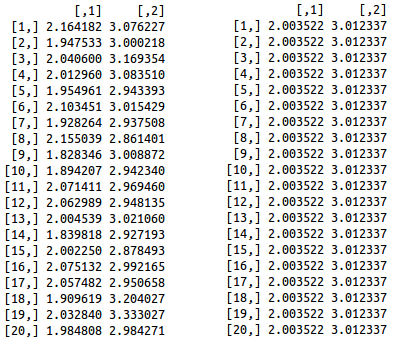
\includegraphics[width=0.4\textwidth]{fig/matrixlabel}
			\caption{Left: example of \texttt{copynumber} matrix for 2 samples. Right: example of the associated \texttt{segmented} matrix.}
		\end{figure}
		
		
		This function returns a list with the same elements as \texttt{segmentData} and some supplementary elements:
		\begin{itemize}
			\item \textbf{calls} A matrix, of the same size as \texttt{copynumber} matrix, containing the label of each point.
			\item \textbf{segment} A data.frame that sums up all the segments found.
			\item \textbf{probdloss} (if you ran \texttt{callingProcess} with \texttt{nclass}=5) A matrix of the same size as \texttt{copynumber} matrix. It contains the probability for each segmented copy-number to be a double loss.
			\item \textbf{probloss} A matrix of the same size as \texttt{copynumber} matrix. It contains the probability for each segmented copy-number to be a loss.
			\item \textbf{probdnorm} A matrix of the same size as \texttt{copynumber} matrix. It contains the probability for each segmented copy-number to be normal.
			\item \textbf{probdgain} A matrix of the same size as \texttt{copynumber} matrix. It contains the probability for each segmented copy-number to be a gain.
			\item \textbf{probdamp} (if you have run \texttt{callingProcess} with \texttt{nclass}=4 or 5) A matrix of the same size as \texttt{copynumber} matrix. It contains the probability for each segmented copy-number to be an amplification.

		\end{itemize}
		
		A wrapper is provided for creating the \texttt{segmentData} argument:
		\begin{verbatim}	
		callingObject(copynumber, segmented, chromosome, position, featureNames, sampleNames)
		\end{verbatim}
		The parameters \texttt{featureNames} and \texttt{sampleNames} can be omitted.		
		
		The following lines continue the example of the section \ref{sec:seg}. They create the \texttt{segmentData} list and run the calling process:
		
\begin{Schunk}
\begin{Sinput}
> #create the segmentData object
> callobj= callingObject(copynumber=seg$signal, segmented=seg$segmented,
+  chromosome=rep(20,length(seg$signal)), position=seg$startPos, 
+  sampleNames="sample1")
> #run the calling
> call=callingProcess(callobj,nclass=3,cellularity=1,verbose=TRUE)
> call$segment
\end{Sinput}
\end{Schunk}
		
		The result of the calling can be seen in figure \ref{callsoutput}.
		
		\begin{figure}[!h]
			\centering
			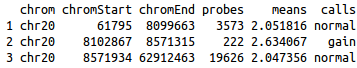
\includegraphics[width=0.5\textwidth]{fig/callsoutput2}
			\caption{The summation of all the segments after running the function \texttt{callingProcess}.}
			\label{callsoutput}
		\end{figure}
		~~\\				
		A wrapper \texttt{CNAobjectToCGHcallObject} to convert CNA object from DNAcopy package \cite{DNAcopy} (CBS segmentation) to the desired format (see \texttt{segmentData}) is also provided.
		
		\begin{verbatim}
			CNAobjectToCGHcallObject(CNAobject)
		\end{verbatim}
		
		\begin{center}
			\begin{tabular}{|l|l|}
				\hline
				Parameters & Description\\
				\hline
				\texttt{CNAobject} & Output of the \texttt{segment} function from \texttt{DNAcopy} package.\\
				\hline	
			\end{tabular}		
		\end{center}
		
		
		\subsection{\texttt{filterSeg} function}
			
			At the end of the calling process, if you have a lot of segments, you might want to filter some uninteresting segments. The \texttt{filterSeg} function allows to filter segments from 3 criteria: the  length in bp, the size in probes and the calling.
			
			\begin{verbatim}
				filterSeg(segmentList,minLength=1,minProbes=1,normalFilter=TRUE)
			\end{verbatim}
			
			\begin{tabular}{|l|l|}
				\hline
				Arguments & Description\\
				\hline
				\texttt{segmentList} & A data.frame containing a description of segments, it must have at least columns:\\
				~ & ``chromStart'', ``chromEnd'', ``probes'' and ``calls'' (see the output of\\
				~ & \texttt{cnSegLabelProcess} and \texttt{callingProcess} functions).\\
				\texttt{minLength} & The minimum length (in bp) for a segment. All the shorter segments are removed.\\
				\texttt{minProbes} & The minimum number of probes for a segment.\\
				~ & All the segments with less probes are removed.\\
				\texttt{keptLabel} & Vector of label to keep. \\
        ~ & Only segment with one of the specified label will be kept.\\
				\hline			
			\end{tabular}
			
			~~\\
			
			It returns a data.frame of the same format as \texttt{segmentList} without the filtered segments.\\
			
			We assume to have a data.frame called \texttt{call\$segment} containing the columns plot in Fig. \ref{callsegplot}
			\begin{figure}[!h]
				\centering
				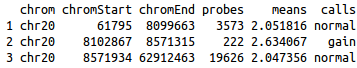
\includegraphics[width=0.5\textwidth]{fig/callsoutput2}
				\caption{\texttt{call\$segment} before filtering.}
        \label{callsegplot}
			\end{figure}
			
			The following command executes the code to keep only segments presenting a gain.
\begin{Schunk}
\begin{Sinput}
> segmentfilter=filterSeg(call$segment,keptLabel="gain")
> segmentfilter
\end{Sinput}
\end{Schunk}
			
			Obtained results are shown in Fig. \ref{filterplot}
			\begin{figure}[!h]
				\centering
				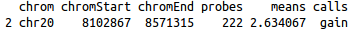
\includegraphics[width=0.5\textwidth]{fig/segapresfiltre2}
				\caption{Result of the filtering.}
        \label{filterplot}
			\end{figure}
	
			
\section{Selection of genomic markers}
	\label{sec:select}
	
	
	In this section, the goal is to select some relevant markers according to a response.\\
	
It consists in minimizing $g_{\lambda}:\beta \in \mathbb{R}^P\mapsto g(\beta)$, where
    \begin{align*}
      g_{\lambda}(\beta) = \sum\limits_{i=1}^I (y_i-(X\beta)_i)^2+\lambda
      \sum\limits_{p=1}^P |\beta_p|  \enspace,
    \end{align*}
      
with $(X\beta)_{i}=\sum_p x_{i,p}\beta_p$ and $\lambda>0$ controlling the number of non-zero coordinates of $\beta$.
%
After minimization, non-zero coefficients $\beta_p$ correspond to influential positions to predict the response. \\
	
	To solve this problem, we use by default the LARS algorithm \cite{lars} that solves the lasso problem for all the values of $\lambda$. In order to choose the best solution, we use a cross validation to select the best values of $\lambda$ and return the associated solution.\\
  
  The spike and slab method \cite{spikeslab1}\cite{spikeslab2} is another alternative in this case of linear regression. It is a three steps procedure including filtering, marker effect estimation and marker selection steps. The filter and marker effect estimation steps use the spike and slab algorithm whereas the marker selection step relies on the elastic net (mixing a $l_1$ penalty whit a $l_2$ penalty). The spike and slab algorithm solves a generalized ridge regression problem ($l_2$ penalty). It is implemented in the R package \texttt{spikeslab} \cite{spikeslabR}. 
	
	\subsection{From data normalized by aroma}	

		The function \texttt{markerSelection} will extract the data from the aroma architecture and run the LARS algorithm and the cross-validation for each chromosome separately.
	
		\begin{verbatim}
markerSelection(dataSetName,dataResponse,chromosome,signal,normalTumorArray,onlySNP,nbFolds,
loss,plot,pkg,...)
		\end{verbatim}
	
	
		\begin{center}
			\begin{tabular}{|l|l|}
				\hline
				Parameters & Description\\
				\hline
				\texttt{dataSetName} & The name of the data-set folder.\\
				\texttt{dataResponse} & A csv files or a data.frame with 2 columns: ``files'' and ``response''.\\
				~ & The column ``files'' contains the filename to extract and\\
				~ &   the second column the response associated with the file.\\
				\texttt{chromosome} & A vector containing the number of the chromosomes for the SNPs selection.\\
				\texttt{signal} & ``CN'' or ``fracB'', corresponding to which signal will be analyzed (default=``CN'').\\
				\texttt{normalTumorArray} & Only in the case of normal-tumor study. A csv file or a data.frame\\
			~~ & containing the mapping between normal and tumor files(Fig. \ref{normalTumorArray}).\\
				\texttt{onlySNP} & Only if \texttt{signal="CN"}. If TRUE, only the SNPs probes are used (default=FALSE).\\
				\texttt{nbFolds} & Number of folds for the cross-validation (default=10).\\
				\texttt{loss}  & either ``logistic'' (binary response) or ``linear'' (quantitative response), default is ``logistic''.\\
				\texttt{plot} & If TRUE, cross-validation mean squared error is plotted (default=TRUE).\\
        \texttt{pkg} & Either ``HDPenReg'' or ``spikeslab''. Used package in linear case (default=``HDPenReg'').\\
				\texttt{...} & supplementary arguments for \texttt{cv.glmnet} function \cite{glmnet} in case of \\
				~ & logistic loss or for \texttt{HDlars} function for linear loss.\\
				\hline	
			\end{tabular}		
		\end{center}
	
		For \texttt{signal="fracB"}, the selection of markers is done for the tumor allele B fraction.
	 
		The function returns a list containing as many elements as the number of chromosomes specified in parameters. The name \texttt{chrX}, where $X$ is the number of a chromosome. Each element of this list is a list containing:
	
		\begin{itemize}
			\item \textbf{chr} The chromosome corresponding to the signal.
			\item \textbf{markers.index} A vector containing the index of all selected markers.
			\item \textbf{markers.position} A vector containing the position of all selected markers.
			\item \textbf{markers.names} A vector containing the name of all selected markers.
			\item \textbf{coefficient} A vector containing the coefficients ($\hat{\beta}$) of all selected markers.
			\item \textbf{intercept} Intercept of the model.

			%\item \textbf{fraction} The fraction of the l1 norm of coefficient selected by cross validation.
		\end{itemize}
		~~\\
	
		For the following example, we assume that the architecture is already created and the data-set is preprocessed as in the previous examples (see section \ref{arch} and \ref{norm}). The response is stored in a data.frame named \texttt{dataResponse} (see Fig. \ref{dataresponse}). 
		
		\begin{figure}[!h]
			\centering
			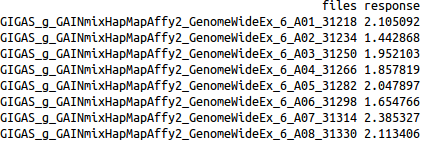
\includegraphics[width=0.5\textwidth]{fig/dataResponse}
			\caption{Example of \texttt{dataResponse} parameters for the \texttt{markerSelection} function.}
			\label{dataresponse}
		\end{figure}
		
The relevant markers can be selected by executing the following code:			
	
\begin{Schunk}
\begin{Sinput}
> dataResponse=data.frame(files=getListOfFiles("datatest1"),
+ response=c(2.105092,1.442868,1.952103,1.857819,2.047897,1.654766,2.385327,2.113406))
> res=markerSelection(dataSetName="datatest1",dataResponse,chromosome=21:22,signal="CN",
+ onlySNP=TRUE,loss="linear")
\end{Sinput}
\end{Schunk}
	
	Figure \ref{SNPoutput} shows the output of the function.
		\begin{figure}[!h]
			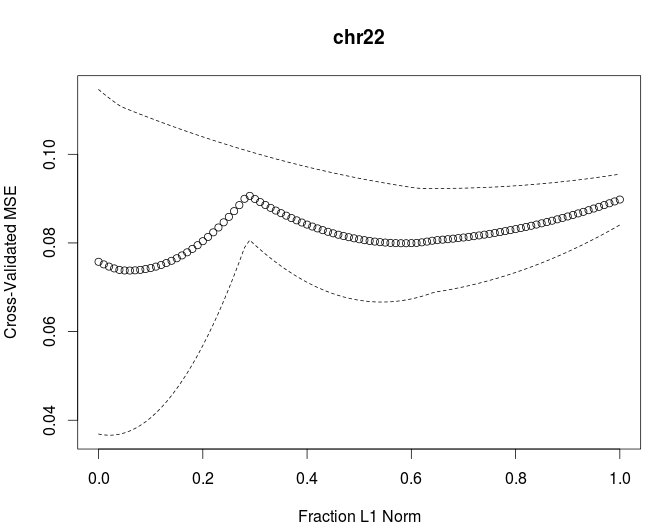
\includegraphics[width=0.5\textwidth]{fig/cvcourbe}
			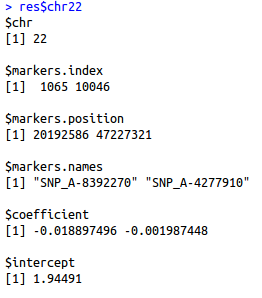
\includegraphics[width=0.3\textwidth]{fig/snpselectres}
			\caption{Left: cross-validation mean squared error. Right: results for chromosome 22.}
			\label{SNPoutput}
		\end{figure}

		In this example, two markers are selected: the 1065th and 10046th markers of the profile (markers.index) at positions 20192586 pb and 47227321 pb on the chromosome 22. The coefficient associated with each selected marker are given in the coefficient vector.

	\subsection{For any data provided in matrices}	

		A version of the selection of markers without the aroma architecture is available:
		
		\begin{verbatim}
			variableSelection(dataMatrix,dataResponse,nbFolds,loss,plot,pkg)
		\end{verbatim}
		
		\begin{center}
			\begin{tabular}{|l|l|}
				\hline
				Parameters & Description\\
				\hline
				\texttt{dataMatrix} & A matrix containing the data, each row is a different signal.\\
				\texttt{dataResponse} & A vector containing the response associated with each signal.\\
				\texttt{nbFolds} & Number of folds for the cross-validation (default=10).\\							
        \texttt{loss}  & either ``logistic'' (binary response) or ``linear'' (quantitative response), default is ``logistic''.\\
				\texttt{plot} & If TRUE plot cross-validation mean squared error (default=TRUE).\\
        \texttt{pkg} & Either ``HDPenReg'' or ``spikeslab''. Used package in linear case (default=``HDPenReg'').\\
				\texttt{...} & supplementary arguments for \texttt{cv.glmnet} function \cite{glmnet} in case of \\
				~ & logistic loss or for \texttt{HDlars} function for linear loss.\\
				\hline	
			\end{tabular}		
		\end{center}

		The output of the functions is:
		
		\begin{itemize}
			\item \textbf{variable} A vector containing the index of all selected markers.
			\item \textbf{coefficient} A vector containing the coefficients ($\hat{\beta}$) of all selected variables.
			\item \textbf{intercept} Intercept of the model.
			%\item \textbf{fraction} The fraction of the l1 norm of coefficient selected by cross validation.
		\end{itemize}
		
		For example, simulate a data-set and the associated response	
\begin{Schunk}
\begin{Sinput}
> dataMatrix=matrix(rnorm(5000,0,0.5),nrow=50)
> dataResponse=drop(dataMatrix%*%sample(c(rep(0,90),rep(1,10))))
> res=variableSelection(dataMatrix,dataResponse,nbFolds=5,loss="linear",plot=TRUE)
\end{Sinput}
\end{Schunk}

  \subsection{To go further}
    In the current implementation of the \texttt{MPAgenomics} R package, two variable selection methods are proposed: $(i)$ the Spike and Slab strategy consisting in first filtering variables to keep most reliable ones, second estimating the effect of remaining variables, and third selecting variables (using AIC), or $(ii)$ Lasso + 10-fold cross validation and elbow search \cite{coude} to choose the unknown parameter $\lambda$ (default choice).\\
  
    In order to compare the two approaches, we have carried out a small simulation study that is shortly described in what follows and mainly summarized by Figure \ref{fig:truefalse}. We run the two approaches with 100 samples generated according to the following design: 
  \begin{itemize}
		\item $I=100$ individuals and $P=1000, 2000,\dots, 10000$ variables
		\item $\beta^* \in \mathbb{R}^p$, the true sparse estimates with only $K=10$ non-zero coefficients
		\item $X\in \mathcal{M}_{I,P}(\mathbb{R})$, $X_1,\dots,X_I \sim \mathcal{N}(0_P,I_P)$
		\item $\epsilon\in\mathbb{R}^P$ Gaussian noise, $\epsilon_1,\dots,\epsilon_I \sim \mathcal{N}(0,\sigma^2)$ with $\sigma^2=0.5$
		\item $y=X\beta^*+\epsilon$
	\end{itemize}	

For each approach, the selected variables were compared to the truth (non-zero elements of $\beta^*$), the average number of true and false selected variables were plotted in Figure \ref{fig:truefalse}. We can see that the \textit{lars} procedure selects here more true variables -- especially when $P$ grows -- and less false variables than \textit{spikeslab}.\\

%We can see (Fig. \ref{fig:truefalse}) that the current procedure in \texttt{MPAgenomics} (\textit{lars} + 10-fold cross validation) outperforms the \textit{spikeslab} procedure in term of variable selection. 

	\begin{figure}[!h]
		\centering
		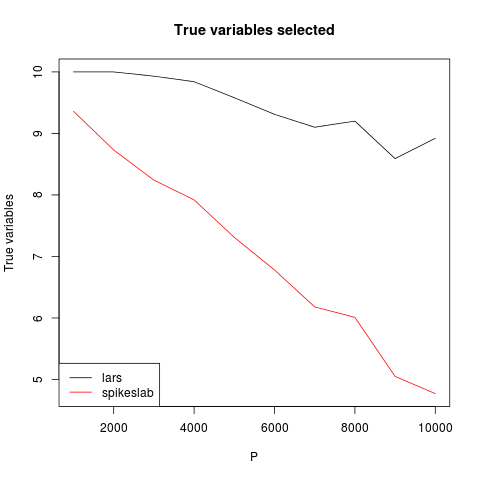
\includegraphics[width=0.37\textwidth]{fig/truesel}
		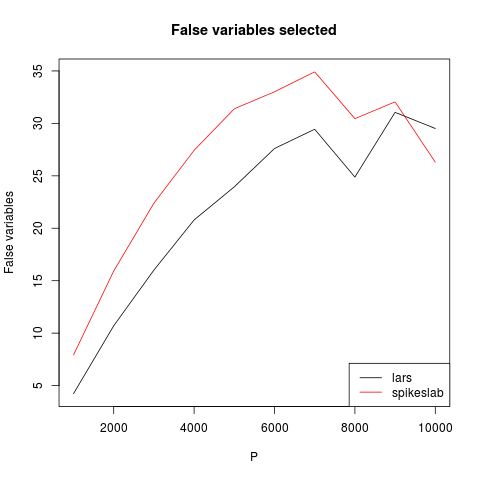
\includegraphics[width=0.37\textwidth]{fig/falsesel}
		\caption{Number of true (Left figure) and false (Right figure) variables selected by two different methods: $(i)$ Lars and 10-fold cross-validation (\textit{lars}), $(ii)$ Spike and Slab (\textit{spikeslab}).}
		\label{fig:truefalse}
	\end{figure}
	
\nocite{*}
\bibliographystyle{apalike}
\newpage

\bibliography{MPAgenomics} 	
\end{document}
